\documentclass{beamer}
\usepackage{booktabs}
%\usepackage{amsmath}
%\usepackage{pdfpages}
%\pdfpagelayout{2 on 1}[letterpaper,border shrink=5mm]

\mode<presentation>
{
%  \usetheme{Malmoe}
\usetheme{Warsaw}
\usecolortheme{seahorse}
  % or ...

 \setbeamercovered{transparent}
  % or whatever (possibly just delete it)
 \setbeamertemplate{footline}[default]
 \setbeamertemplate{navigation symbols}{\insertslidenavigationsymbol\insertframenavigationsymbol\insertdocnavigationsymbol}
}

\title{IQC Validator}

%\subtitle{Include Only If Paper Has a Subtitle}

\author{NCATS Informatics}
%\author{Dac-Trung Nguyen}
% - Give the names in the same order as the appear in the paper.
% - Use the \inst{?} command only if the authors have different
%   affiliation.

%\institute[NCATS] % (optional, but mostly needed)
%{National Center for Advancing Translational Sciences}
% - Use the \inst command only if there are several affiliations.
% - Keep it simple, no one is interested in your street address.

\date[]% (optional, should be abbreviation of conference name)
{December 9, 2013}

\begin{document}

\begin{frame}
  \titlepage
\end{frame}

\begin{frame}
\frametitle{Overview}
\begin{itemize}
\item Desktop client
\item Proposed scoring function to evaluate data fitting
\end{itemize}
\end{frame}

\begin{frame}
\frametitle{Desktop client}
\framesubtitle{Features}
\begin{itemize}
\item A simple desktop client to help validate the CYP isozyme data
  generation workflow 
\centerline{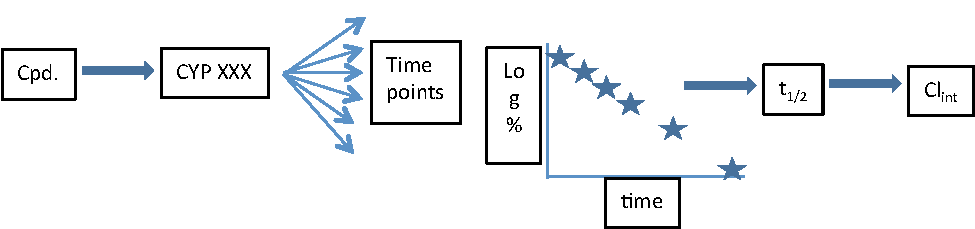
\includegraphics[width=3.5in]{iqc-flow}}
\item Minimal user interaction
\begin{itemize}
  \item Precalculate results for all possible combinations
  \item Rank results based on scoring function
\end{itemize}
\item A web-based protocol for data management (i.e., data upload,
  download, and annotation)
\item Available at
\centerline{\href{http://tripod.nih.gov/ws/iqc/iqc.jnlp}{\texttt{http://tripod.nih.gov/ws/iqc/iqc.jnlp}}}
\end{itemize}
\end{frame}

\begin{frame}
\frametitle{Desktop client (cont'd)}
\framesubtitle{Screenshot}
\centerline{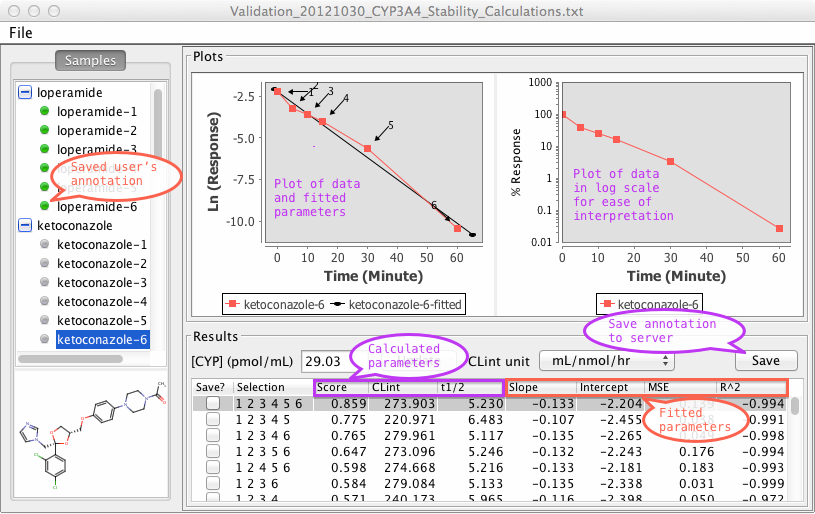
\includegraphics[width=4in]{iqc-validator}}
\end{frame}

\begin{frame}
\frametitle{Proposed scoring function}
\begin{itemize}
\item Developed based on discussion with Scott Obach and Ed Kerns
\item Let the raw score be defined as follows
\begin{equation}
\textrm{Score}_{\textrm{raw}} = NR^2\exp(-\sigma_e)\sum_i 2^{-i},
\end{equation}
where $N$ is the number of data points used to build the linear model,
$\sigma_e \ge 0$ and $R \in [-1,1]$ are the estimated mean square
error and Pearson's correlation of the model, respectively. 
\item Weighted contribution of $T_0, T_5, T_{10}, T_{15}, T_{30},
  T_{60}$ as $1, \frac{1}{2}, \frac{1}{4},
  \frac{1}{8},\frac{1}{16},\frac{1}{32}$, respectively.
\item The best possible raw score (i.e., $\sigma_e = 0$, $|R| = 1$, and
  $N = 6$) is 
\[ \textrm{Score}_{\textrm{best}} = 6\sum_{i=0}^5 2^{-i} = 11.8125\]
with $i$ corresponds to the index of $\left\{T_0,T_5, T_{10},
  T_{15}, T_{30}, T_{60}\right\}$.
\end{itemize}
\end{frame}

\begin{frame}
\frametitle{Scoring function (cont'd)}
\begin{itemize}
\item Normalized score is the ratio of raw and best
\[ \textrm{Score} = \frac{\textrm{Score}_{\textrm{raw}}}%
{\textrm{Score}_{\textrm{best}}}\]
where Score $\in [0, 1]$.
\item Initial observations
\begin{itemize}
\item Good fit when score $\ge 0.9$
\item In good agreement with with manual evaluation (based on limited
  annotations from Ed Kerns)
\end{itemize}
\item Require additional validation
\begin{itemize}
\item Collect additional manual annotations 
\item Evaluation metric (e.g., Spearman's rank correlation)
\end{itemize}
\end{itemize}
\end{frame}
\end{document}
